\documentclass{beamer}
\usepackage[utf8]{inputenc}
\usepackage[T1]{fontenc}
\usepackage[portuges,brazilian]{babel}
\usepackage{graphicx}
\usepackage[sfdefault]{quattrocento}
\usepackage{multicol}
\usepackage{hyperref}
\usetheme[showheader,blue,colorblocks]{Verona}
\title{JPEG 2000}
\subtitle{Sistemas Multimídia}
\author[Yuri, Joel]{Yuri Oliveira \and Joel Rocha}
\institute[IFCE]{Instituto Federal de Ciência, Arte e Tecnologia}
\date{Dezembro, 2015}
\logo{
\includegraphics[width=0.8cm]{figure/logo.jpg}}
\begin{document}
\begin{frame}
\titlepage
\end{frame}
\begin{frame}{\contentsname}
\tableofcontents
\end{frame}
\section{Introdução}
\begin{frame}{Introdução}
   \begin{itemize}
      \item Comprimir é necessário!
      \item Fotografias, páginas WEB, exames médicos.
      \item Facilitar o armazenamento e transmissão.
      \item Permite usar imagens menores com mesmo efeito.
      \item Considere uma imagem...
         \begin{itemize}
            \item Tamanho: 3 in x 4 in (7,62 cm x 10,16 cm)
            \item Resolução: 500 dpi
            \item Pixel: 3 bytes
            \item 3.000.000 pixels = 9.000.000 bytes = \textbf{9 MB} (7 disquetes)
         \end{itemize}
   \end{itemize}
\end{frame}
\subsection{Compressão de dados}
\begin{frame}{Compressão de dados}
   \begin{block}{\textit{Lossless}}
      \begin{itemize}
         \item Sem perda de dados.
         \item Maior processamento.
         \item Permite reconstrução.
         \item Desenhos técnicos, textos, quadrinhos, mapas.
         \item \emph{Run-lengh encoding} (Huffman, LZW).
         \item PNG, GIF, TIFF.
      \end{itemize}
   \end{block}
\end{frame}
\begin{frame}{Compressão de dados}
   \begin{block}{\textit{Lossy}}
      \begin{itemize}
         \item Com perda de dados.
         \item Maior compressão.
         \item Não permite reconstrução.
         \item Fotografia em geral.
         \item Descarta o que é imperceptível.
         \item JPEG, PGF, ICER.
      \end{itemize}
   \end{block}
\end{frame}
\subsection{JPEG 1992}
\begin{frame}{JPEG 1992}
   \begin{block}{Relembrando}
      Método de compressão de imagens com perda de dados que usa a transformada discreta do cosseno (DCT) e obtém o resultado assumindo que altas frequências não são percebidas.
   \end{block}
\end{frame}
\section{JPEG 2000}
\subsection{Melhorias}
\begin{frame}{JPEG 2000}
   \begin{block}{Melhorias:}
      \begin{itemize}
         \item \emph{Lossy} e \emph{Lossless}
         \item Wavelet
         \item Melhor compressão: Alta qualidade e Lossy (20\% a 200\%).
         \item Várias resoluções.
         \item \emph{Region of Interest} (ROI).
         \item Transmissão progressiva.
         \item Resistência a erros.
         \item Formato do arquivo flexível.
      \end{itemize}
   \end{block}
\end{frame}
\begin{frame}{JPEG versus JPEG 2000}
   \begin{multicols}{2}
   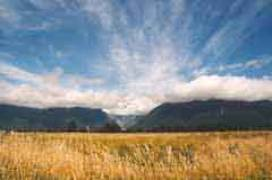
\includegraphics[width=0.5\textwidth]{figure/ex_jpeg_01.jpg}
   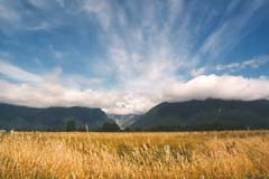
\includegraphics[width=0.5\textwidth]{figure/ex_jpeg2k_01_2.jpg}
   \end{multicols}
\end{frame}
\begin{frame}{JPEG versus JPEG 2000}
   \begin{multicols}{2}
   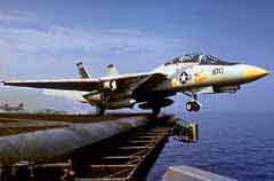
\includegraphics[width=0.5\textwidth]{figure/ex_jpeg_02_1.jpg}
   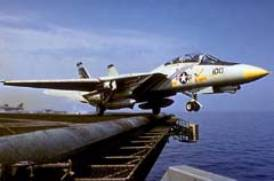
\includegraphics[width=0.5\textwidth]{figure/ex_jpeg2k_02_2.jpg}
   \end{multicols}
\end{frame}
\subsection{Como funciona?}
\begin{frame}{Como funciona?}

\end{frame}
\begin{frame}{Wavelet}
   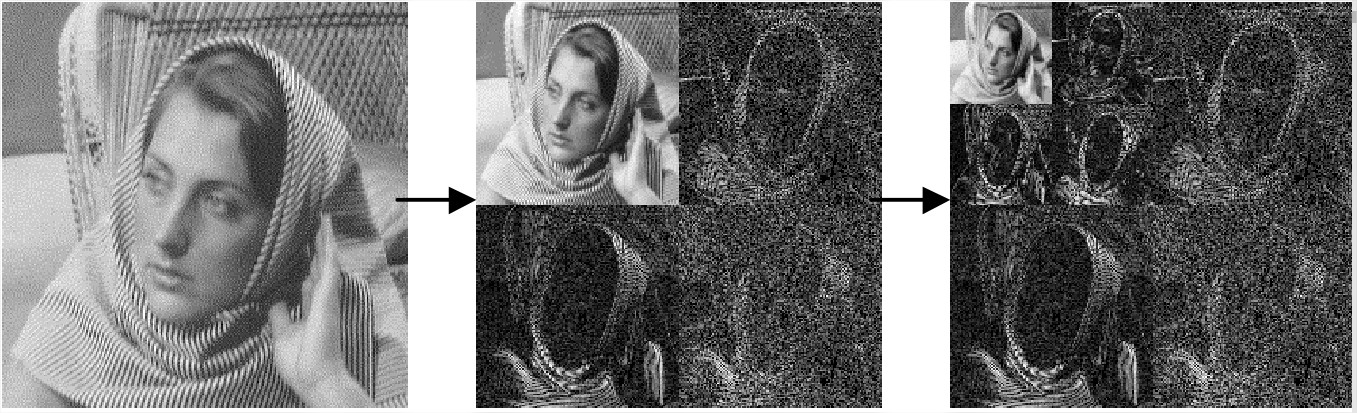
\includegraphics[width=\textwidth]{figure/wavelet-1.jpg}
\end{frame}
\section{Análise dos resultados}
\subsection{Critério}
\begin{frame}{Relação sinal-ruído de pico}
   \begin{block}{Definição}
      PSNR, \emph{Peak Signal-to-Noise Ratio}, define a relação entre energia máxima de um sinal e o ruído que afeta a representação dele.

      $$ PSNR(dB) = -20 \log \frac{RMSE}{2^b -1} $$

      $RMSE$ é o erro quadrático médio e $b$ é a quantidade de \emph{bits}.
   \end{block}
\end{frame}
\subsection{Ferramenta}
\begin{frame}{Ferramentas}
   \begin{tabular}{| l | l | l |}
      \hline
      \textbf{Nome} & \textbf{Tipo} & \textbf{Descrição} \\
      \hline
      LuraWave JP2 & JPEG2000 & Comercial \\
      \hline
      Jasper & JPEG2000 & Não comercial, mais usado \\
      \hline
      BOI & JPEG2000 & Não comercial, Java. \\
      \hline
      HD Photo Device Porting Kit & HD Photo & JPEG2000 da Microsot \\
      \hline
      IrfanView JPEG & JPEG & JPEG da IrfanView \\
      \hline
   \end{tabular}
\end{frame}
\subsection{Casos de teste}
\begin{frame}{Babuíno}
   \begin{multicols}{2}
      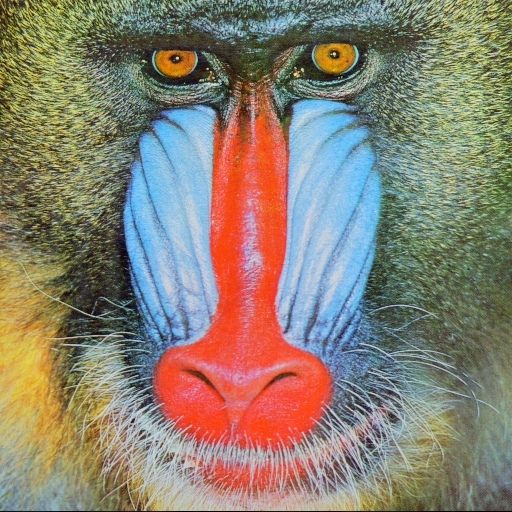
\includegraphics[width=0.5\textwidth]{figure/baboon100.jpg}
      \begin{itemize}
         \item Tamanho: 786 486 bytes
         \item Resolução: 512 x 512
         \item Imagem colorida com muitos detalhes - pêlo e bigodes. Difícil de comprimir, pois contém uma grande variação de cor e uma grande quantidade de textura.
      \end{itemize}
   \end{multicols}
\end{frame}
\begin{frame}{Farol}
   \begin{multicols}{2}
      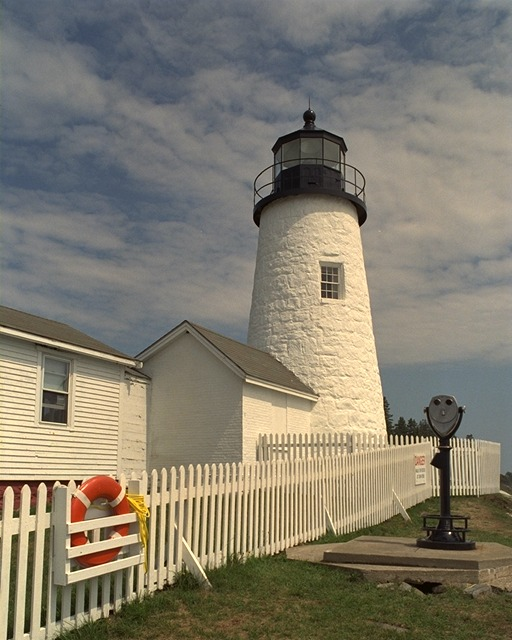
\includegraphics[width=0.45\textwidth]{figure/lighthouse100.jpg}
      \begin{itemize}
         \item Tamanho: 983 094 bytes
         \item Resolução: 512 x 640
         \item Imagem colorida com muitos detalhes como cerca e corrimão na parte superior do farol. Também mostra o céu.
      \end{itemize}
   \end{multicols}
\end{frame}
\begin{frame}{Barbara}
   \begin{multicols}{2}
      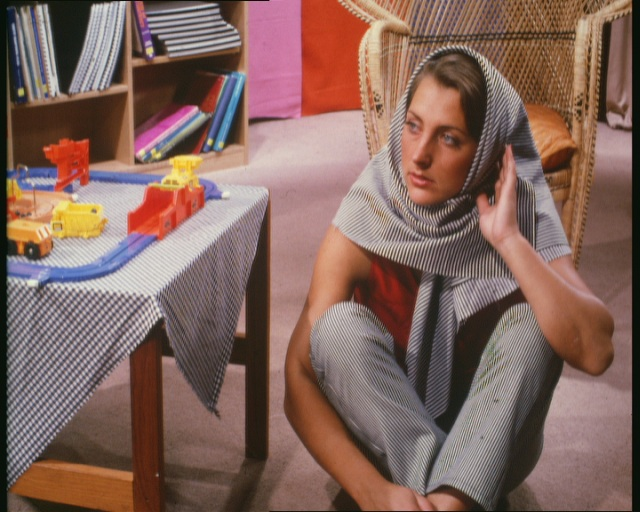
\includegraphics[width=0.5\textwidth]{figure/barbara100.jpg}
      \begin{itemize}
         \item Tamanho: 983 094 bytes
         \item Resolução: 640 x 512
         \item Imagem colorida. Rosto humano básico e pele.
      \end{itemize}
   \end{multicols}
\end{frame}
\subsection{Resultados}
\begin{frame}
   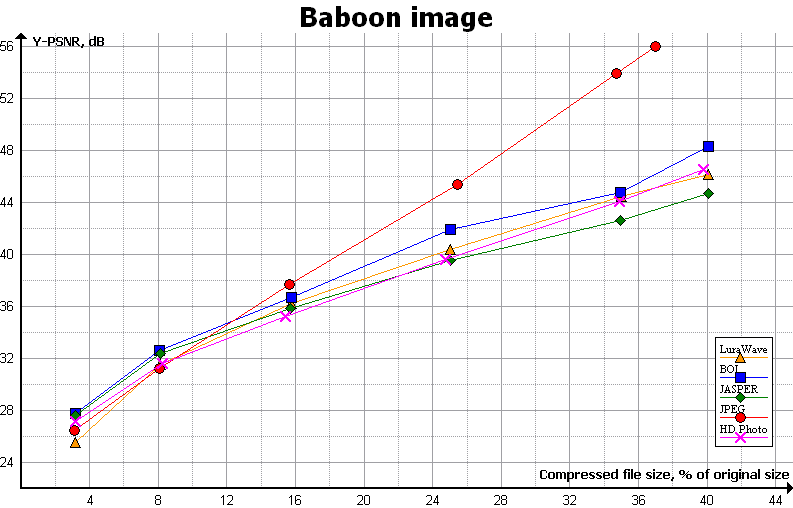
\includegraphics[width=\textwidth]{figure/baboon_psnr.png}
\end{frame}
\begin{frame}{JPEG 2000 (BOI)}
   \begin{multicols}{2}
      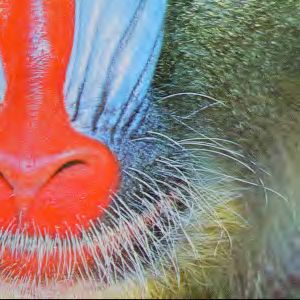
\includegraphics[width=0.5\textwidth]{figure/BOI_baboon030.jpg}
      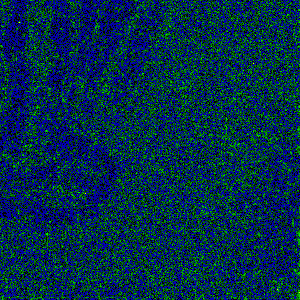
\includegraphics[width=0.5\textwidth]{figure/psnr_BOI_baboon030.png}
   \end{multicols}
\end{frame}
\begin{frame}{JPEG}
   \begin{multicols}{2}
      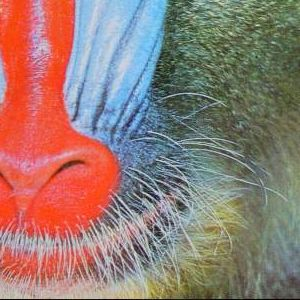
\includegraphics[width=0.5\textwidth]{figure/JPEG_baboon030.jpg}
      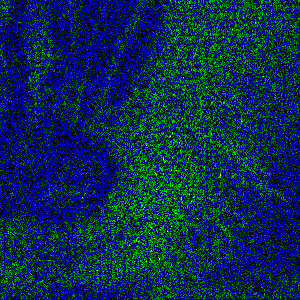
\includegraphics[width=0.5\textwidth]{figure/psnr_JPEG_baboon030.png}
   \end{multicols}
\end{frame}
\begin{frame}
   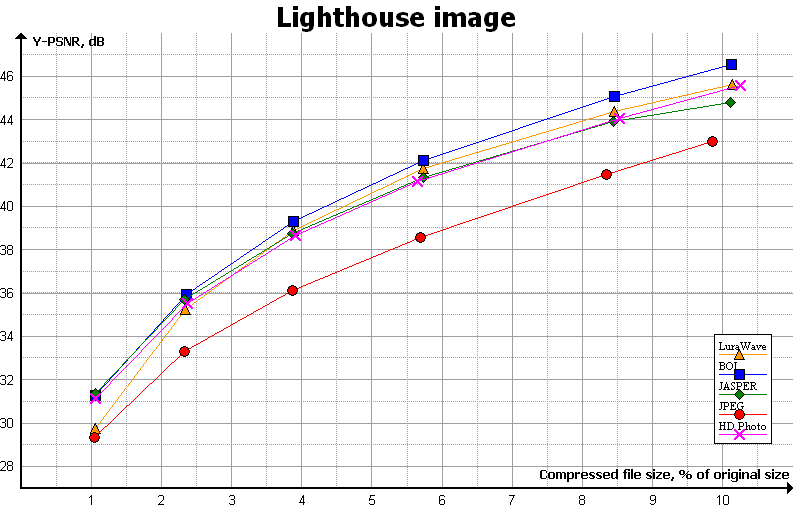
\includegraphics[width=\textwidth]{figure/lighthouse_psnr.png}
\end{frame}
\begin{frame}{JPEG 2000 (BOI)}
   \begin{multicols}{2}
      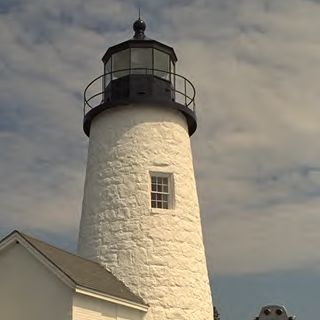
\includegraphics[width=0.5\textwidth]{figure/BOI_lighthouse050.jpg}
      
\includegraphics[width=0.5\textwidth]{figure/psnr_BOI_lighthouse050.png}
   \end{multicols}
\end{frame}
\begin{frame}{JPEG}
   \begin{multicols}{2}
      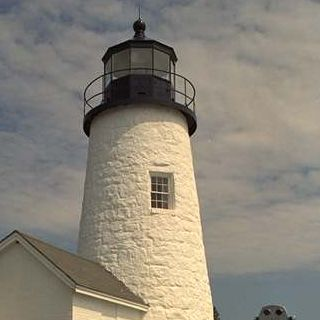
\includegraphics[width=0.5\textwidth]{figure/JPEG_lighthouse050.jpg}
      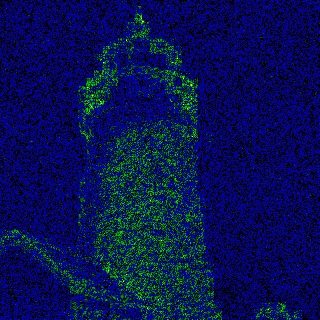
\includegraphics[width=0.5\textwidth]{figure/psnr_JPEG_lighthouse050.png}
   \end{multicols}
\end{frame}

\begin{frame}
   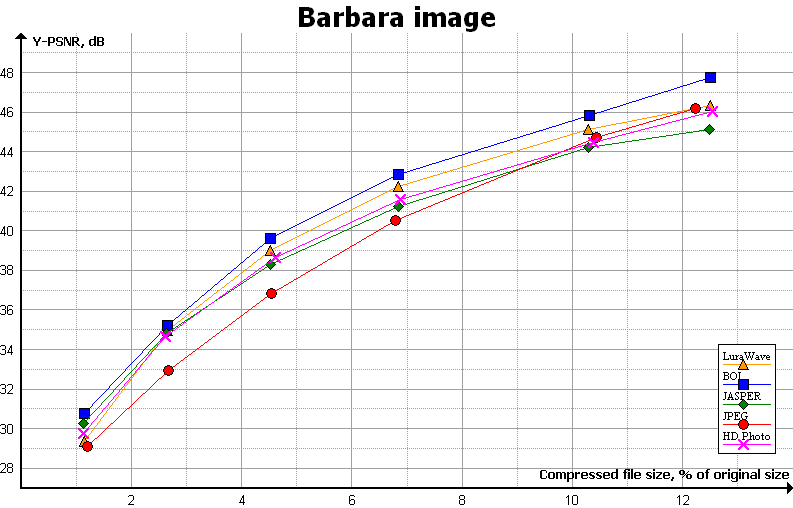
\includegraphics[width=\textwidth]{figure/barbara_psnr.png}
\end{frame}
\begin{frame}{JPEG 2000 (BOI)}
   \begin{multicols}{2}
      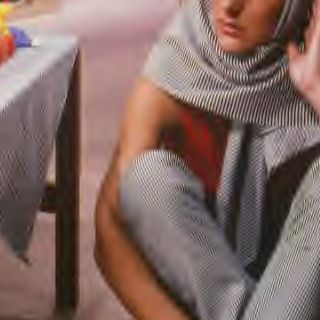
\includegraphics[width=0.5\textwidth]{figure/BOI_barbara010.jpg}
      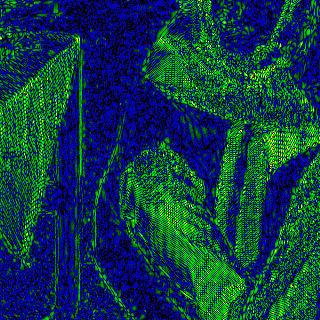
\includegraphics[width=0.5\textwidth]{figure/psnr_BOI_barbara010.png}
   \end{multicols}
\end{frame}
\begin{frame}{JPEG}
   \begin{multicols}{2}
      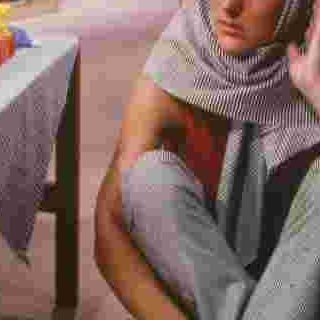
\includegraphics[width=0.5\textwidth]{figure/JPEG_barbara010.jpg}
      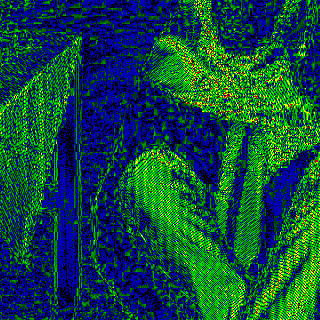
\includegraphics[width=0.5\textwidth]{figure/psnr_JPEG_barbara010.png}
   \end{multicols}
\end{frame}


\section{Implementação}
\section{Referências}
\begin{frame}{Referências}
   \begin{itemize}
      \item \href{https://en.wikipedia.org/wiki/JPEG_2000}{JPEG 2000 - Página do Wikipédia.}
      \item \href{http://stefan.winklerbros.net/Publications/adip2004.pdf}{EBRAHIMI, CHAMIK, WINKLER. JPEG vs. JPEG2000: An Objective Comparison of Image Encoding Quality.}
      \item \href{http://faculty.gvsu.edu/aboufade/web/wavelets/student_work/EF/}{ELZINGA, FEENSTRA. JPEG 2000: The Next Compression Standard using wavelet technology.}
      \item \href{http://www.mvnet.fi/index.php?osio=Tutkielmat&luokka=Yliopisto&sivu=Image_compression}{VESTOLA. A study about image compression.}
      \item \href{http://web.stanford.edu/class/ee398a/handouts/papers/Christopoulos\%20-\%20JPEG2000.pdf}{CHRISTOPOULOS, SKODRAS, EBRAHIMI. The JPEG2000 Still Image Coding: An Overview.}
   \end{itemize}
\end{frame}

\end{document}
